\chapter{Theoretical Framework}
\section{Sequential Decision-Making}
In robotics, sequential decision-making problems refers to tasks in which a robot must achieve a goal by physically interacting with the environment, for example, navigating from one point to another, grasping an object, balancing, etc. It can be described as a step-by-step decision theory, where depending on the information that is gathered by its sensors, the robot has to make decisions consecutively.

\subsection{Markov Decision Process (MDP)}
A Markov Decision Process (MDP) is meant to be a straightforward framing of sequential decision-making problems. In a MDP we have an \emph{agent} and an \emph{environment}, which interact continually. The agent is the learner and the decision maker. The environment is everything that the agent can interact with\cite{sutton}. In robotics, the agent is the robot and the environment is the setting, in the real world, in which the robot interacts.

To keep things as simple as possible, MDPs are commonly modeled as discrete time interaction of the agent with the environment. Thus, the time is divided into a sequence of \emph{time steps}, $t=0,1,2,3,...$ . At each time step the agent \emph{observes} $o_{t}$ a representation of the environment's \emph{state} $s_{t}$. Depending on the state, the agent selects an \emph{action} $a_{t}$, that, ideally, will lead to achieving the goal of the task.

The state describes the current situation of the environment; the action is an input to the environment that the agent can select and that affects the environment's evolution. The agent receives a representation of the state which is called the observation. In robotics, this is information gathered with sensors such as RGB cameras, encoders, inertial measurement units, etc. If the observation contains sufficient information such that the agent can fully understand the environment state, then the problem is said to be \emph{fully observed}, otherwise, is called \emph{partially observed}. If a partially observed problem is modeled with a MDP, then is called a partially observable MDP, or POMDP.

The environment's evolution is the sequence of states visited by the agent. Transitioning from one state to another is a stochastic process defined by the nature of the environment and the actions taken, at each time step, by the agent. Additionally, a MDP is formulated as an extension of a Markov chain, such that the Markov property is satisfied. As a consequence, the conditional probability distribution of future states depends only upon the present state, such that:

\begin{equation}
    p(s_{t}|s_{t-1}, a_{t-1}) = p(s_{t}|s_{t-1},...,s_{0},a_{t-1},...,a_{0})  \hspace{0.5cm} \forall t
\end{equation}

Finally, every time the environment transitions, a numerical \emph{reward} is received by the agent. Better decisions will produce higher rewards.

In a nutshell, a MDP can by defined by the tuple $MDP=(\mathcal{S},\matchcal{A},\mathcal{R},\mathcal{P})$, where $\mathcal{S}$ represents the state space and $\mathcal{A}$ the action space. $\mathcal{R}$ represents the \emph{reward function}, which generates a scalar reward $r$ every time step. This reward may depend on $s_{t-1}$; $s_{t-1},a_{t-1}$ or $s_{t-1},a_{t-1},s_{t}$, so $\mathcal{R}$ can be defined with $\mathcal{R}: \mathcal{S} \to \R$, $\mathcal{R}: \mathcal{S} \times \mathcal{A} \to \R$ or $\mathcal{R}: \mathcal{S} \times \mathcal{A} \times \mathcal{S} \to \R$, respectively. Finally, $\mathcal{P}$ corresponds to the transition function, which is the probability $p(s_{t+1}|s_{t}, a_{t})$, where $\mathcal{P}: \mathcal{S} \times \mathcal{A} \times \mathcal{S} \to [0, 1]$. Graphically, a MDP can be summarized in the following diagram:

\begin{figure}[H]
    \centering
    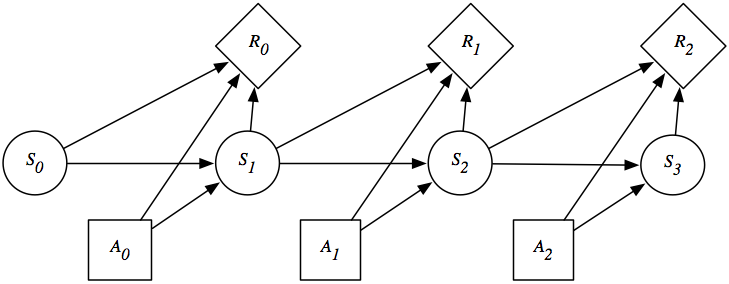
\includegraphics[width=0.7\linewidth]{imagenes/cap1/mdp.png}
    \caption{Finite part of a Markov Decision Process.}
    \label{fig:msim}
\end{figure}

\section{Reinforcement Learning}
Reinforcement Learning aims to use the MDP framing of sequential decision-making problems so that agents learn to solve tasks from \emph{experience}. In this case, experience is understood as the agent-environment interaction (see Figure \ref{fig:agent-environment}), which results in the generation of reward values that indicates the quality of the decisions made by the agent. 

\begin{figure}[h]
    \centering
    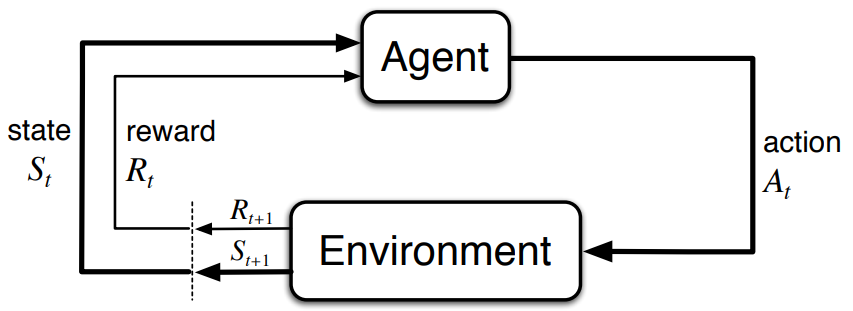
\includegraphics[width=0.7\linewidth]{imagenes/cap1/agent_environment.png}
    \caption{The agent-environment interaction.}
    \label{fig:agent-environment}
\end{figure}

The idea is to use this experience to learn/discover a \emph{policy} that maximizes the total amount of reward the agent receives. A policy $\pi$ is a function that maps states into actions in a deterministic $\pi: \mathcal{S} \to \mathcal{A}$ or stochastic $\pi: \mathcal{S} \times \mathcal{A} \to [0,1]$ manner. To obtain a good performing policy, is necessary to adequately combine \emph{exploration} with \emph{exploitation}. When exploring, the agent finds more information about the environment, when exploiting, it exploits known information to maximize the reward.

Commonly, in complex problems, $\pi$ is a parametrized model; then, the goal of reinforcement learning is to find the set of parameters $\theta$ that maximizes the sum of rewards, or \emph{return} $G$, that the agent will obtain when solving a task. As a consequence of the parametrized policy $\pi_{\theta}$, the agent will follow a trajectory $\tau = \{s_{0}, a_{0},...,s_{T}, a_{T}\}$, where $T$ is the number of time steps. When a problem has well-defined initial and final conditions it has a \emph{finite horizon} (the trajectory generated between the initial and final conditions is called \emph{episode}), otherwise, it has an \emph{infinite horizon}. In the former, $T \in \N$; in the later, $T \to \infty$. Finally, $\tau$ follows the probability distribution $p_{\theta}(\tau)$ that depends on $p(s_{t+1}|s_{t}, a_{t})$, $\pi_{\theta}$ and $p_{0}=p(s_{0})$, which corresponds to the initial distribution of states.

Then, the goal of reinforcement learning is to \textbf{maximize the expected return} of a given task such that:

\begin{equation}
    J = E_{\tau \sim p_{\theta}(\tau)} \left[\sum_{t=0}^{T}r(s_{t}, a_{t})\right]
\end{equation}

\begin{equation}
    \theta^{*} = \argmax_{\theta}J(\theta)
\label{eq:objective}
\end{equation}

It can be observed that in the infinite horizon case, this definition can be numerically unstable and have divergence problems. To address this, the term $\gamma \in [0, 1)$ can be introduced to construct a formulation of the goal with \emph{discounted rewards}:

\begin{equation}
    J = E_{\tau \sim p_{\theta}(\tau)} \left[\sum_{t=0}^{T}\gamma^{t}r(s_{t}, a_{t})\right]
\end{equation}

$\gamma$ allows to control the horizon in which the agent maximizes the reward.

\newpage

\subsection{Learning Policies}

Under this framework, there are different approaches for learning policies:

\begin{itemize}
    \item Value Based (Critic)
    \item Policy Based (Actor)
    \item Actor-Critic
\end{itemize}

In the \textbf{Value Based} approach, the policy is learnt implicitly by learning a \emph{value function}. This function estimates the expected return of the agent for every state, or in other words, how good is to be in a given state. The value for a given state will depend in the in policy of the agent, thus, the value function can be written as:

\begin{equation}
    V^{\pi}(s_{t'})  = E_{\tau' \sim p_{\theta}(\tau')}\left[\sum_{t=t'}^{T}\gamma^{t}r_{t}(s_{t}, a_{t})|s_{t'}\right]
\end{equation}

Where $\tau'$ is the trajectory followed by the agent starting from time step $t'$.

Similarly, the value of taking the action \emph{a} in the state \emph{s} can be estimated by a function, which is called the \emph{action-value function}:

\begin{equation}
    Q^{\pi}(s_{t'}, a_{t'})  = E_{\tau' \sim p_{\theta}(\tau')}\left[\sum_{t=t'}^{T}\gamma^{t}r_{t}(s_{t}, a_{t})|s_{t'},a_{t'}\right]
\end{equation}

The main idea is to find a policy $\pi^{*}$, which is called the \emph{optimal policy}, such that:

\begin{equation}
    V^{\pi^{*}}(s) \geq V^{\pi}(s) \hspace{0.5cm} \forall s, \pi
\end{equation}

\begin{equation}
    Q^{\pi^{*}}(s,a) \geq Q^{\pi}(s,a) \hspace{0.5cm} \forall s,a,\pi
\end{equation}

If these conditions are met, then $\theta^{*}$ is obtained. On the other hand, \textbf{Policy Based} approaches update $\theta$ by direct policy differentiation. In this case, the challenge is to estimate the gradient of $J(\theta)$ to update $\theta$ iteratively, using gradient ascent:

\begin{equation}
    \Delta \theta = \alpha \nabla_{\theta}J(\theta)
\end{equation}

\begin{equation}
    \theta \leftarrow \theta + \Delta \theta
\end{equation}

Where $\alpha$ is the learning rate.

Finally, \textbf{Actor-Critic} approaches combine Value Based and Policy Based methods. Figure \ref{fig:rl_summ} summarizes these RL approaches:

\begin{figure}[h]
    \centering
    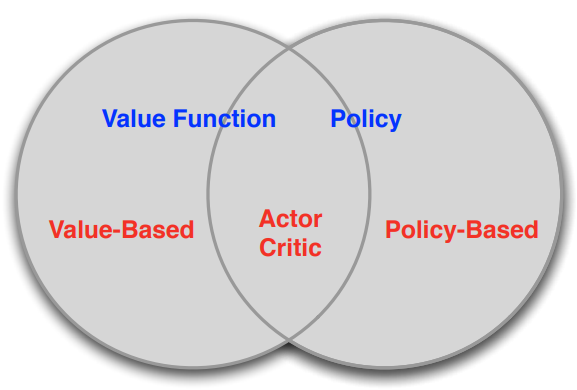
\includegraphics[width=0.5\linewidth]{imagenes/cap1/rl_summary.png}
    \caption{Reinforcement Learning methods.}
    \label{fig:rl_summ}
\end{figure}

Independently of the technique that is used to solve a problem with Reinforcement Learning, the anatomy these algorithms is always the same: obtain experience (generate samples), fit a model (or estimate a return), improve the policy and repeat (see Figure \ref{fig:RL_anatomy}). 

\begin{itemize}
    \item \textbf{Generate samples:} obtain $n$ transitions. A transition is the quadruple $(s_{t}, a_{t}, r_{t+1}, s_{t+1})$, which can also be written as $(s, a, r, s')$.
    \item \textbf{Fit a model:} use the gathered samples to improve the estimation of a value function or to estimate $\nabla_{\theta} J(\theta)$.
    \item \textbf{Improve the policy:} use the estimated value function to obtain a policy or $\nabla_{\theta} J(\theta)$ to update $\theta$.
\end{itemize}

\begin{figure}[h]
    \centering
    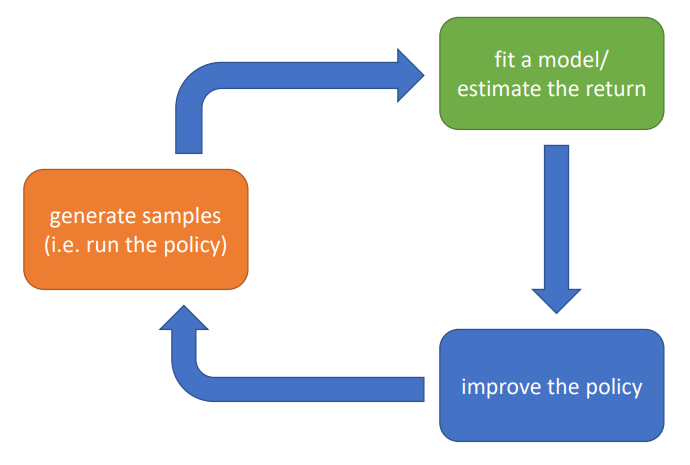
\includegraphics[width=0.7\linewidth]{imagenes/cap1/RL_anatomy.png}
    \caption{Anatomy of Reinforcement Learning.}
    \label{fig:RL_anatomy}
\end{figure}

\subsubsection{Model-Free vs Model-Based}
Reinforcement Learning approaches may be either Model-Free or Model-Based.

\textbf{Model-Free} algorithms learn a policy directly from experience. The dynamics of the environment are not directly learned.

\textbf{Model-Based} algorithms learn a \emph{model} of the dynamics of the environment from experience. Then, planning or optimal control techniques are applied to develop a policy using the model.

A model of the environment is a function $M: \mathcal{S} \times \mathcal{A} \to \mathcal{S}$ that predicts the next state as a function of the current state and action to take:

\begin{equation}
    M(s_{t},a_{t}) = s_{t+1}  
\end{equation}

or, in the stochastic case, $M: \mathcal{S} \times \mathcal{A} \times \mathcal{S} \to [0, 1]$:

\begin{equation}
    M(s_{t},a_{t}) = p(s_{t+1}|s_{t},a_{t})  
\end{equation}

Figure \ref{fig:free_based_model} summarizes the difference between both approaches:

\begin{figure}[h]
    \centering
    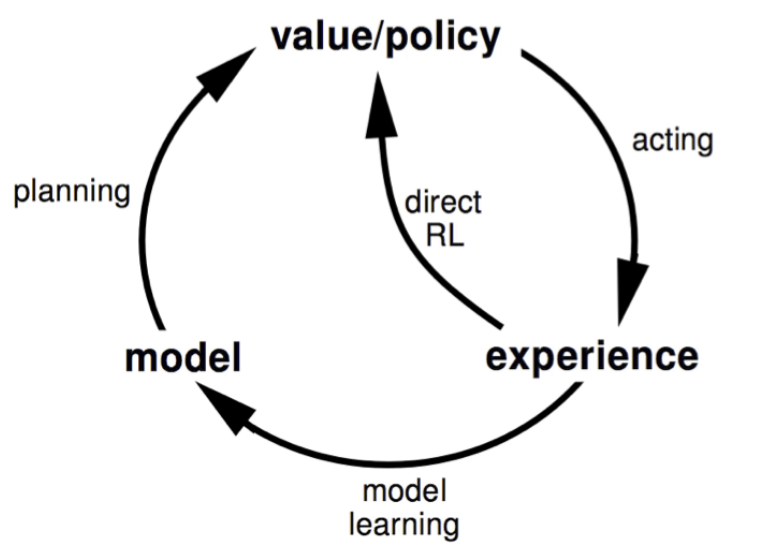
\includegraphics[width=0.6\linewidth]{imagenes/cap1/free_based_model.png}
    \caption{Model-Free vs Model-Based.}
    \label{fig:free_based_model}
\end{figure}

\subsubsection{Experience Replay}
The anatomy of Reinforcement Learning (Figure \ref{fig:RL_anatomy}) suggests that every time the policy is improved, is necessary to obtain new samples in order to improve it again. This is only true in \emph{on-policy} algorithms. On-policy algorithms are those in which a policy can only be updated with data gathered by itself. Data gathered before the last update corresponds to data gathered by a past version of the current policy; thus, gathered by a different policy. So if the policy is changed, even a little bit, is necessary to generate new samples. 

On the other hand, \emph{off-policy} algorithms are able to improve a policy without the aforementioned restriction; thus, using samples collected by other policies or by past versions of itself. Under this context is where is useful to use \emph{experience replay}.

The key idea of experience replay is to store old transitions $(s, a, r, s')$ in a buffer (or memory buffer) and replay them constantly (randomly sampling a mini-batch) when updating a policy. Using experience replay have two advantages: (1) the data/samples are uncorrelated and (2) data efficiency is significantly improved:

\begin{itemize}
    \item \textbf{Uncorrelated samples:} every sequential decision-making problem has the issue that the data generated when exploring the environment is correlated. If the data is correlated, then, every time the policy is updated, this will be with respect to a sequence, or various sequences. In some cases this is problematic because models may locally overfit to this data, constantly forgetting older experiences. This issue can be tackled by randomly sampling from a memory buffer.
    
    \item\textbf{Data efficiency:} depending on the the parametrized model of $\pi_{\theta}$, it may not be efficient to update its parameters with a set of samples just once. To successfully extract all the information contained in the samples, it would be necessary to update the model several times from them. This is achieved when using experience replay.
\end{itemize}

\section{Function Approximation}
Although $\pi$ can be represented by a lookup table, where every state has a corresponding action stored in a table, this representation is not scalable to complex problems with large state/action spaces. This is mainly because the states and/or actions are too many to be stored in memory and/or it would take too long to adequately explore the states. Thus, in robotics contexts, where state/action spaces are most likely continuous, the standard approach is to use function approximation. As mentioned before, this means that the policy is a parametrized model $\pi_{\theta}$.

There is a large list of different function approximators, but in this work two of them are the most relevant: \textbf{linear models of basis functions (LCBFs)} and \textbf{artificial neural networks (ANNs)}. Although the policy may not be directly represented by these models, as in the case of value function approximation, for simplicity, from now on we are going to assume that it always does. Also, we are only going to work with deterministic policies. So, if the function approximator is $\Psi$, then $\pi_{\theta} = \Psi(s;\theta)$ such that $\Psi: \mathcal{S} \to \mathcal{A}$.

\subsection{Linear Model of Basis Functions}
A well-known case of function approximation in RL is that in which $\pi_{\theta}$ is a linear function of
the weight vector $\theta$. Specifically, we are going to work with linear combinations of gaussian radial basis functions (RBFs). If $\phi(s)$ corresponds to a vector of basis functions which is weighted by $\theta$, then $\pi_{\theta}$ can be represented as:

\begin{equation}
    \pi_{\theta}(s) = \phi(s) \cdot \theta
    \label{eq:lcbf}
\end{equation}

In this case, $\phi(s)$ corresponds to normalized gaussians:

\begin{equation}
    \phi'_{i}(s) = \exp\left( -\frac{1}{2}[s - c_{i}]B^{-1}_{i}[s-c_{i}]\right) 
    \hspace{1cm}
    \phi_{i}(s) = \frac{\phi'_{i}(s)}{\sum_{i'=1}^{N}{\phi'_{i'}(s)}}
\end{equation}

Where $N$ is the number of basis functions and the subindex $i$ refers to the i-th basis function.

\subsection{Artificial Neural Networks}

ANNs are a widely used model for non-linear function approximation. The idea behind these models is to build a network of interconnected units that have some properties inspired on neurons. There is a large variety of models, the ones relevant to this work are the following:

\begin{itemize}
    \item Feedforward Fully-Connected
    \item Convolutional
    \item Autoencoder
    \item Recurrent
\end{itemize}

\subsubsection{Feedforward Fully-Connected}
    
Feedforward Fully-Connected or Feedforward neural networks (FNNs) are the quintessential ANN model. These models are called to be feedforward because the information flows in one sense from the input, trough intermediate representations, to the output. In the mathematical formalization, a network is understood as the model generated when many functions are composed. For instance, you may have three functions ($f^{(1)}$, $f^{(2)}$, $f^{(3)}$) connected in a chain such that:

\begin{equation}
    \Psi(s) = f^{(3)}(f^{(2)}(f^{(1)}(s)))
\end{equation}

Each of these functions represents a \emph{layer}, the overall number of layers is known as the \emph{depth} of the neural network. Commonly, these layers have $n\mathrm{-dimensional}$ outputs, and each dimension of the outputs corresponds to the output of a single \emph{neuron}. A neuron is a function $h$ composed by weights $w$, a bias $b$ and a nonlinear function $\sigma$, known as the activation function:

\begin{equation}
    h(x) = \sigma(w \cdot x + b)
    \label{eq:h}
\end{equation}

There are different types of activation functions, such as ReLU, sigmoid or hyperbolic tangent \textbf{CITE}. Graphically, this function is described in Figure \ref{fig:neuron}.

\begin{figure}[H]
    \centering
    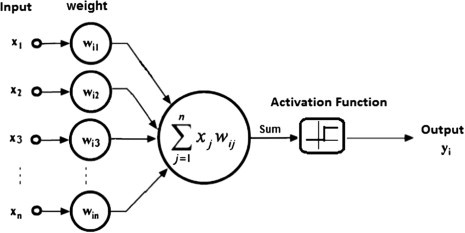
\includegraphics[width=0.6\linewidth]{imagenes/cap1/neuron.jpeg}
    \caption{Neuron ($b$ considered as an extra dimension of $w$).}
    \label{fig:neuron}
\end{figure}

As mentioned before, a layer have many neurons, the number of neurons in a layer is known as the \emph{width} of the layer. The inputs $x$ of a neuron are the outputs of every neuron of the past layer.  There are three types of layers: \textbf{input}, \textbf{hidden} and \textbf{output}. The input layer is the input of $\Psi$, which is $s$ in this context (which is not actually a layer). The output layer is the final function in the chain of functions that compose $\Psi$, which outputs the output of $\Psi$. And finally, the hidden layers are all the functions in between the input and output layers. Graphically, a FNN with one hidden layer is presented in Figure \ref{fig:FNN}, where every layer is denoted by $u_{j}$.

\begin{figure}[H]
    \centering
    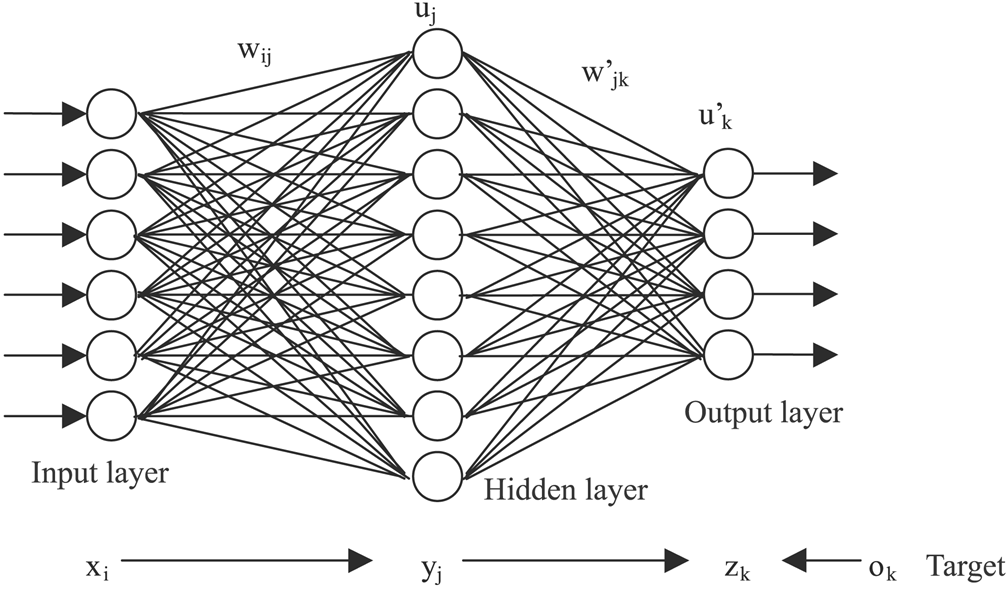
\includegraphics[width=0.6\linewidth]{imagenes/cap1/NeuralNetwork.png}
    \caption{Feedforward Neural Network model with one hidden layer.}
    \label{fig:FNN}
\end{figure}

It can be observed that the nonlinearity that characterizes neural networks exists because of the activation functions, which are nonlinear. This is an essential condition for neural networks to be \emph{universal approximators}. What this states is that a neural network with at least one hidden layer containing a large enough finite number of neurons can approximate any continuous function on a compact region of the network's input space to any degree of accuracy \textbf{CITE sutton 183}. This is a powerful property; nevertheless, finding the set of weights that parametrize the network in order to approximate an arbitrary function is another story, and a lot of work has been done in that regard. 

Finally, going back to the concept of a parametrized policy $\pi_{\theta}$, in this case $\theta$ would correspond to the concatenation of all the weights (including biases) of the layers of a network. \newline

\subsubsection{Convolutional}
    
Convolutional Neural Networks (CNNs) are a specialized type of neural network. The main feature of these networks is that they are designed such that convolutions are employed in at least one layer. In the area of signal processing convolutions are a well-known tool for applying filters to signals, and at the same time, filtering signals is a well-known way of extracting features out of them. The approach proposed by CNNs is to learn the weights of these filters (also known as kernels) as a part of the network's learning process, and that by construction, these filters are applied to the inputs of the convolutional layers.

The way to achieve this is to replace the dot product in Equation \ref{eq:h} by a convolution operation. Usually, in these problems we work with discrete data, so the discrete version of the convolution is used:

\begin{equation}
    s(x)_{i} = (x * w)_{i} = \sum_{l=0}^{L}w_{l} \cdot x_{i+l}
\end{equation}
    
The sub-index $i$ corresponds to the $i\mathrm{-}eth$ term of the input $x$. $w$ corresponds to the kernel, which has dimension $L$. It can be observed that the kernel is applied over a region of each index $i$, which means that this operation cares about the order of the data, and as a consequence, these networks are used with inputs that have spatial or time correlations, such as images or time series. CNNs are widely use for image processing problems, so is often to use convolutions over more than one axis at a time. If we have a two-dimensional image as an input it seems natural to use a two-dimensional kernel $K$ as well (to exploit spatial correlations):

\begin{equation}
    s(x)_{i} = (x * K)_{i} = \sum_{l=0}^{L}\sum_{m=0}^{M}K_{l, m} \cdot x_{i+l, j+m}
\end{equation}

In this case K has dimension $L \times M$. Figure \ref{fig:conv} shows an example of a kernel operation over a pixel.

\begin{figure}[H]
    \centering
    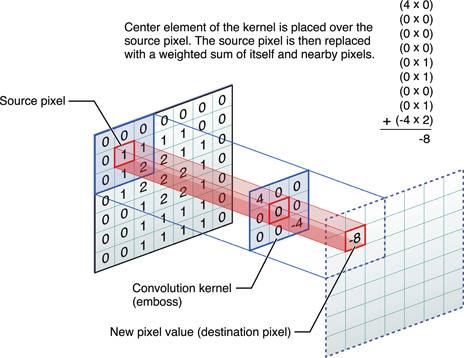
\includegraphics[width=0.4\linewidth]{imagenes/cap1/convolution.jpg}
    \caption{Convolution operation in an image.}
    \label{fig:conv}
\end{figure}

So, in CNNs, Equation \ref{eq:h} has the following shape:

\begin{equation}
    h(x)_{i} = \sigma(s(x)_{i} + b)
    \label{eq:h2}
\end{equation}

Each neuron will correspond to the output of a kernel applied over a region of the input; thus, the output of the full convolution operation will correspond to a set of neurons. As a consequence, the weights, which in this case is the kernel, will be shared between neurons, which does not happens in the FNN case. Is important to note that is also common to apply the convolution operation over images with arbitrary depth. For instance, RGB images have depth=3 (red, green and blue channels), so in these cases filters with arbitrary depth may be used as well. Also, considering the assumption that each filter extracts one kind of feature out of a signal, usually, several filters are applied over an input, where every filter generates a different image (set of neurons) as an output. These means that the depth of the output of a convolutional layer will be equal to the number of filters applied.

To modify the output of a convolutional layer further, is common to use a \textbf{pooling function}. This function summarizes the output of the convolution operations replacing every value of the outputs with a statistic of the nearby outputs. One example of a pooling function is the \emph{max pooling}, which takes the maximum value over a rectangular neighborhood, as it can be seen in Figure \ref{fig:maxpool}. 

\begin{figure}[H]
    \centering
    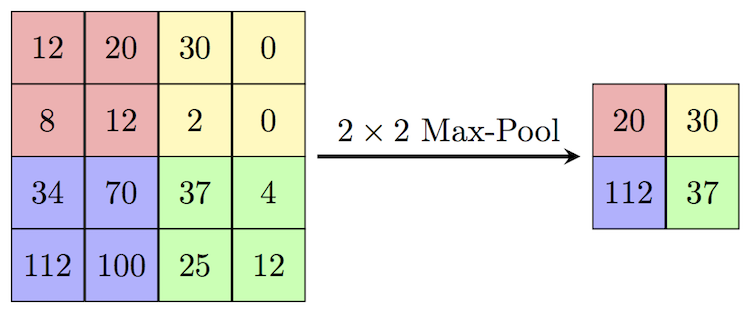
\includegraphics[width=0.4\linewidth]{imagenes/cap1/max_pool.png}
    \caption{Max pooling operation.}
    \label{fig:maxpool}
\end{figure}

Pooling helps the model to be approximately invariant to translations in the input. An alternative to pooling, is to use a convolution with \textbf{stride} greater than one. The stride is the distance skipped between values of the input to where the kernel is applied, which in the default case is one (no skipping). It has been observed that replacing pooling by stride$>1$ has no loss in accuracy for several image recognition benchmarks \cite{springenberg2014striving}. Figure \ref{fig:cnn} shows a CNN used for classification.
    
\begin{figure}[H]
\centering
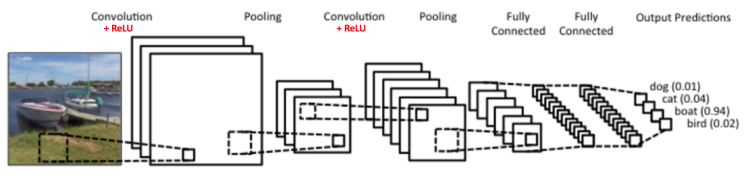
\includegraphics[width=0.9\linewidth]{imagenes/cap1/cnn.png}
\caption{Convolutional Neural Network.}
\label{fig:cnn}
\end{figure}

\subsubsection{Autoencoder}
    
An autoencoder is a special type of ANN that aims to copy the input of the network to its output i.e. aims to be the identity function. Although solving this problem may seem to be useless, it has some interesting properties. In this work, we are interested in using autoencoders for dimensionality reduction and feature learning. 

This neural network is divided in two parts, the \textbf{encoder $e(x)$} and the \textbf{decoder $d(\mathcal{L})$}. When used for dimensiolanity reduction and feature learning, the encoder tries to encode the input into a space of lower dimension (a bottleneck), called the \textbf{latent space $\mathcal{L}$}, which represents a compressed representation of the input $x$, $\mathcal{L}=e(x)$. The decoder takes the latent space and tries to reconstruct the input $\widetilde x = d(\mathcal{L})$, where $\widetilde x$ is the reconstruction of $x$, see Figure \ref{fig:ae}. The objective of using autoencoders in this context is to obtain a latent space that captures the most salient features of the input. 
    
\begin{figure}[H]
    \centering
    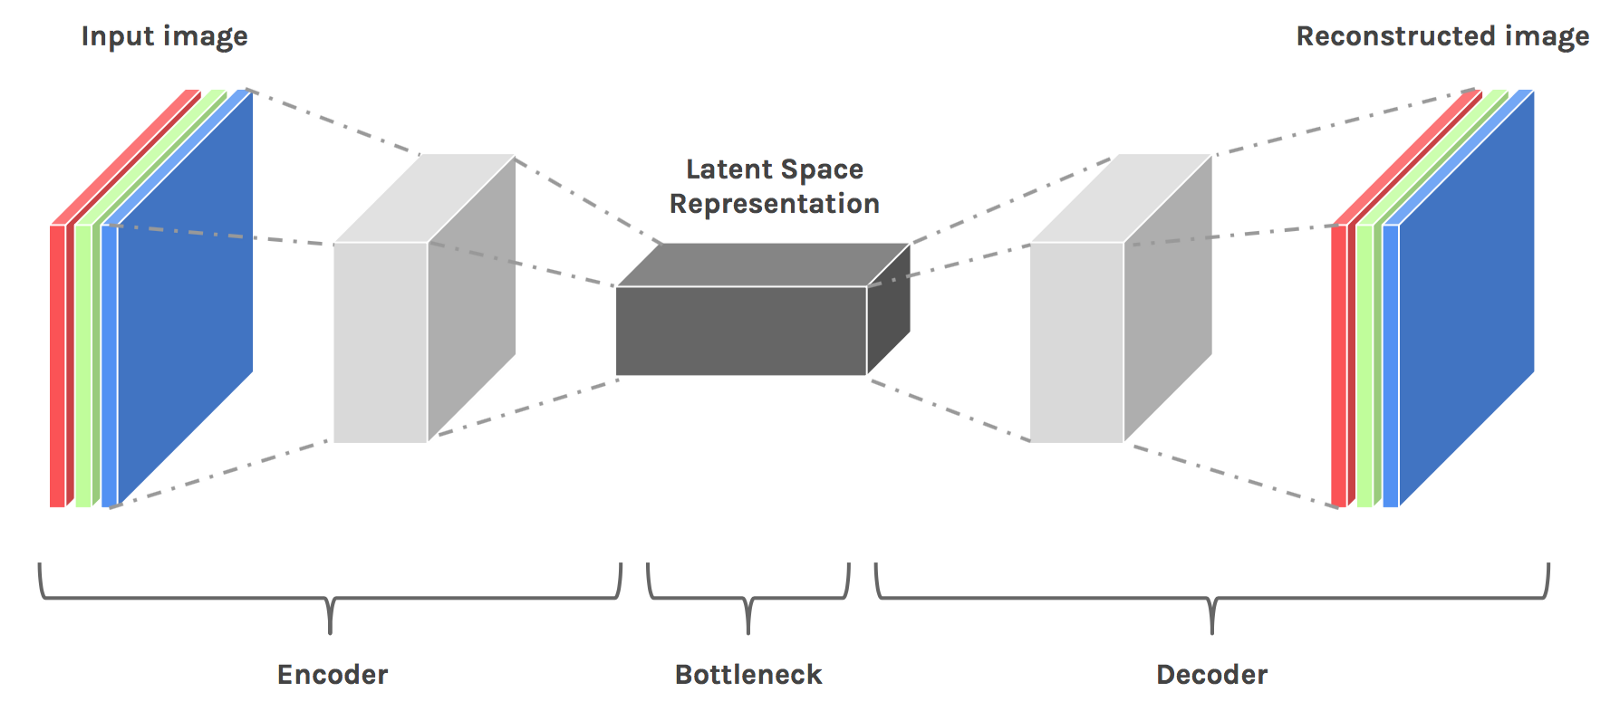
\includegraphics[width=0.8\linewidth]{imagenes/cap1/ae.png}
    \caption{Autoencoder.}
    \label{fig:ae}
\end{figure}
    
The goal of the autoencoder is to minimize the loss function:

\begin{equation}
    L(x, \widetilde x = d(e(x)))
\end{equation}

Where $L$ is a dissimilarity function such as the mean squared error. This model may have convolutional, fully-connected, both or other types of layers.

\subsubsection{Recurrent}
    
Recurrent Neural Networks (RNNs), unlike FNNs or CNNs, have memory. They are designed to work with sequential data. What this means, that past evaluations of the network affect the ones in the future. RNNs have an internal state, or hidden state $h_{state}^{t}$ ($t$ represents the time step), that is modified every time an input is fed to the network such that:

\begin{equation}
    h_{state}^{t} = f(h_{state}^{t-1}, x^{t}; \theta)
\end{equation}

In the \textbf{vanilla} RNN, one of the simplest models of RNNs, a neuron of a recurrent layer is understood as the $i\mathrm{-eth}$ term of the hidden state, $h_{state\mathrm{-}i}^{t}$. If compared with Equation \ref{eq:h}, an RNN neuron has the following structure:

\begin{equation}
    h_{state\mathrm{-}i}^{t}(x) = \sigma(w_{hh} \cdot h_{state\mathrm{-}i}^{t-1} + w_{xh} \cdot x^{t} + b)
\end{equation}

Where the main difference is that the term $w_{hh} \cdot h_{state\mathrm{-}i}^{t-1}$ is incorporated, and the concatenation of the weights $w_{hh}$ and $w_{xh}$ corresponds to $w$. Figure \ref{fig:rnn_unfolded} represents a vanilla RNN in its \emph{unfolded} representation.

\begin{figure}[h]
    \centering
    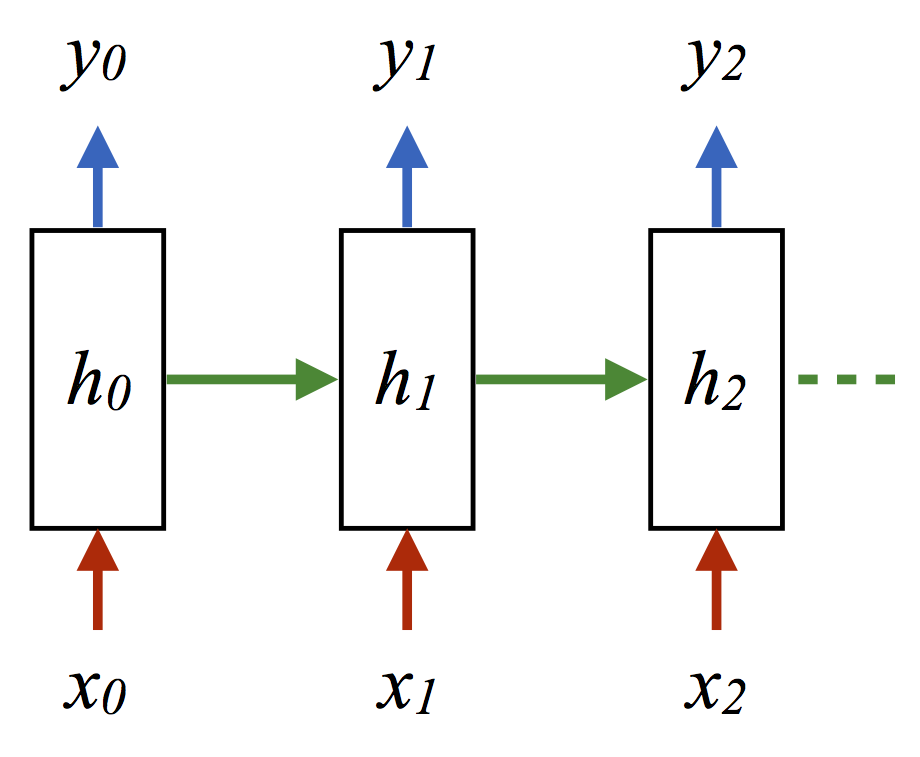
\includegraphics[width=0.3\linewidth]{imagenes/cap1/unfolded_rnn.png}
    \caption{Unfolded vanilla RNN.}
    \label{fig:rnn_unfolded}
\end{figure}


In RNN contexts, commonly, the hidden state is represented as a whole vector directly, and not by the equations of every neuron. A weight matrix $W_{h}$ is used, and corresponds to the concatenation of the weights of every neuron, including the bias, such that:

\begin{equation}
    h_{state}^{t}(x) = \sigma(W_{hh} h_{state}^{t-1} + W_{xh} x^{t}) = \sigma \left(W_{h} \begin{pmatrix} h^{t-1} \\ x^{t} \end{pmatrix} \right)
\end{equation}

In a vanilla RNN with one hidden state, $\sigma$ is the hyperbolic tangent function $tanh$ and one more operation is added to obtain an output $y$:

\begin{equation}
    y^{t}(x) = W_{hy}h_{state}^{t}(x)
\end{equation}

Nevertheless, vanilla RNNs have some structural problems related to the computation of their gradients (exploding and vanishing gradients) \cite{bengio1994learning, pascanu2013difficulty}. So in practice, more complex RNN architectures are used, such as \textbf{Long Short-Term Memory (LSTM)} \cite{hochreiter1997long} or \textbf{Gated Recurrent Unit (GRU)} \cite{cho2014learning} networks. The architecture relevant to this work is LSTM, and one of its layers can be summarized with the following equations:

\begin{equation}
    \begin{pmatrix} i \\ f \\ o \\ g \end{pmatrix} = \begin{pmatrix} \sigma_{f} \\ \sigma_{f} \\ \sigma_{f} \\ tanh \end{pmatrix} W \begin{pmatrix} h^{t-1} \\ x^{t} \end{pmatrix} 
\end{equation}

\begin{equation}
    c^{t} = f \odot c^{t-1} + i \odot g
\end{equation}

\begin{equation}
    h^{t} = o \odot tanh(c^{t})
\end{equation}

Where $i$, $f$, $o$, $g$ are called \textbf{gates} and each one of them is a vector used for internal computations of the recurrent unit. $\sigma_{f}$ corresponds to the $sigmoid$ activation function, $\odot$ is the element-wise product (Hadamard product) operator and $W$ is a weight matrix containing the submatrices $W_{i}$, $W_{f}$, $W_{o}$ and $W_{g}$. A LSTM layer or unit has two internal states $c^{t}$ and $h^{t}$. $h^{t}$ is still known as the hidden state and $c^{t}$ is known as the cell state.

\subsection{Parameter Tuning}

Until now, we have discussed that policies can by represented as parametrized models, called function approximators, and that the two most relevant to this work are LCBFs and ANNs. Nevertheless, we have not discussed on how to tune the parameters of these models in order for them to approximate a specific function.

First, is necessary to define a loss function, in this work we use the \textbf{Mean Squared Error (MSE)}, which gives us a measure of how close are the vector outputs generated by our model $\Psi(s;\theta)=\hat{y}$ with respect to observed target values $y$. Then, the objective is to minimize this function in the parameter space with some optimization method, in this case we use \textbf{Stochastic Gradient Descent (SGD)}. Given that this method needs to compute the gradient of the loss function $J(\theta)=MSE(\Psi(\theta))$, is necessary to compute the gradient of $\Psi(\theta)$.

When using LCBFs, this computation is trivial, such that the gradient of \ref{eq:lcbf} woud be:

\begin{equation}
    \nabla_{\theta} \Psi(\theta)_{LCBF} = \phi(s)
\end{equation}

But, in the case of ANNs computing the gradient is not direct. Given that we have a function composed by layers, is necessary to propagate the error through all of these layers in order to update all of the weights of the network. \textbf{Backpropagation} \cite{rumelhart1988learning} is the technique used to achieve this and, in principle, it uses the chain rule to quantify how much changes in past layers affect later ones. Nowadays, there are several computer tools that have this algorithm incorporated and that automatically computes the gradients of ANNs using symbolic math and differentiable programming, such as Tensorflow \cite{tensorflow2015-whitepaper} or PyTorch \cite{paszke2017automatic}.

\subsection{Deep RL Era}

Reinforcement Learning can be divided in the \emph{pre Deep RL era} and the \emph{Deep RL era}, which is the current one. In the year 2012, the first work known of successfully solving sequential decision-making problems with high-dimensional state spaces using CNNs was presented \cite{Mnih2015}. This was a consequence of the new advances that where being made in the area of ANNs or \textbf{Deep Learning (DL)}. When ANNs have several layers, which was the case for the mentioned work, they are called \textbf{Deep Neural Networks (DNNs)}. The area that combines DL with RL is called \textbf{Deep RL}. Deep RL gives agents the possibility to build rich state representations of the environment without feature engineering on the side of the designer, which was always necessary in classical RL. This drew a lot of attention and made Deep RL increasingly popular over the past few years \cite{franccois2018introduction}.

Before the Deep RL era, ANNs where not a predominant function approximator for solving sequential decision-making problems. In the pre Deep RL era, one of the most widely used function approximators were LCBFs, as stated in a survey of the year 2013 \cite{kober2013reinforcement}. 

\section{Interactive Machine Learning}

In the context of this work, Interactive Machine Learning (IML) is understood as a research area that gathers all the techniques in which humans/users take part in the agent's learning process for solving sequential decision-making problems. Other works refer to IML as an area that focuses on learning classifiers with the help of users \cite{fails2003interactive, ware2001interactive, amershi2012regroup, ngo2014efficient}; that is out of the scope of this work.  

As RL, IML can also be studied under the framework of MDPs. The main difference with RL is that in this case having an explicitly defined reward function is not a requirement. Some approaches may combine the information gathered from the human with the one given by a reward function, while others, may not need a reward function at all. Figure \ref{fig:LfF} summarizes the LfF approach.

\begin{figure}[h]
    \centering
    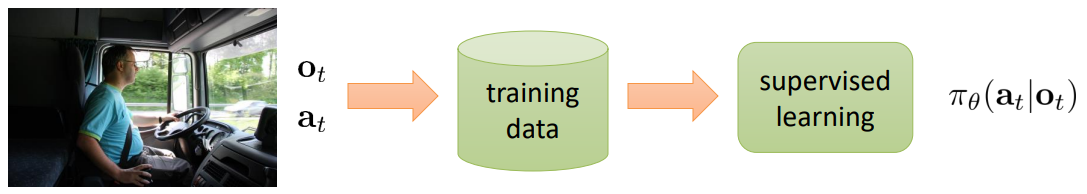
\includegraphics[width=0.9\linewidth]{imagenes/cap1/b_cloning.png}
    \caption{Behavior cloning.}
    \label{fig:b_cloning}
\end{figure}

In this work, we divide IML into two areas: \textbf{Learning from Demonstration (LfD)} and \textbf{Learning from Feedback (LfF)}. 

\subsection{Learning from Demonstration}

LfD is a learning paradigm in which a demonstrator provides labelled data of a desired policy. Then, the agent tries to copy the demonstrator's behavior by shaping its policy in a supervised learning manner, using as database the data provided by the demonstrator (see Figure \ref{fig:b_cloning}). This is the most basic LfD approach and it takes the name of \textbf{Behavior Cloning}.

\begin{figure}[h]
    \centering
    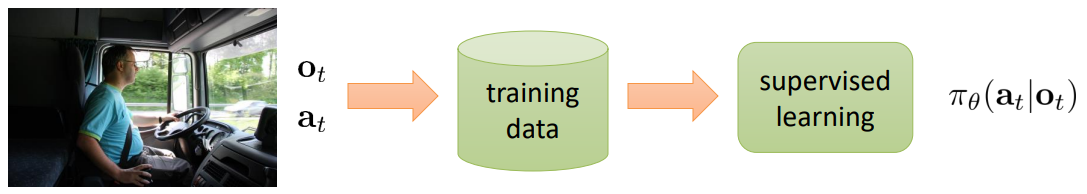
\includegraphics[width=0.9\linewidth]{imagenes/cap1/b_cloning.png}
    \caption{Behavior cloning.}
    \label{fig:b_cloning}
\end{figure}

\subsubsection{Imitation Learning}

When the platform of the agent is different to the one in which the demonstrations are made, we talk about \textbf{Imitation Learning}. In this case, the learning agent must identify a mapping between the demonstrator and itself. This is a setting that arises naturally in real-world problems. For instance, let's suppose that we want to teach a robot how to walk. Using a camera, we could record a human making demonstrations (just by walking), but then, the robot should figure out how to map that observations into labeled data over its own state and action spaces. The problem of identifying this mapping is one of the main difficulties of LfD approaches and is known as \textbf{The Correspondence Problem}.

\subsubsection{Distributional Drift}

The \textbf{Distributional Drift} is an issue that every LfD approach could have if is not taken into account. This problem arises because the probability distribution of the trajectory followed by the policy $p_{\pi_{\theta}}$ "drifts" from the one of the demonstrator $p_{data}$. This happens because even though the agent imitates the demonstrator, is very difficult for the agent to make a perfect imitation. Thus, small errors over several states accumulate into a larger error that eventually makes the agent to fail. This phenomenon can be observed in Figure \ref{fig:drift}, where the drift is shown over one dimension of the state.

\begin{figure}[H]
    \centering
    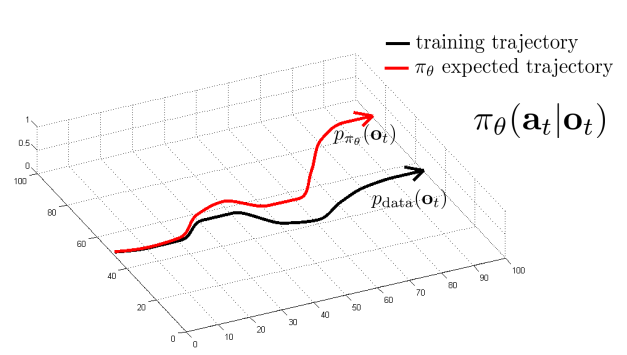
\includegraphics[width=0.7\linewidth]{imagenes/cap1/drift.png}
    \caption{Distributional Drift.}
    \label{fig:drift}
\end{figure}

A well-known algorithm that tackles this problem is called \textbf{DAgger} \cite{ross2011reduction}. This approach matches $p_{\pi_{\theta}}$ with $p_{data}$, such that $p_{\pi_{\theta}} = p_{data}$. The main idea is that instead of collecting samples from the demonstrator, collect them by running $\pi_{\theta}$ and then label them with the demonstrator. Samples are collected, labeled, added to the database $\mathcal{D}$ and used for training iteratively, in order to approach asymptotically to $p_{data}$. The basic structure of DAgger is the following:

\begin{enumerate}
    \item Train $\pi_{\theta}(a_{t}|o_{t})$ from human data $\mathcal{D}=\{o_{1},a_{1},...,o_{T},a_{T}\}$
    \item Run $\pi_{\theta}(a_{t}|o_{t})$ to get dataset $\mathcal{D}_{\pi_{\theta}}=\{o_{1},...,o_{M}\}$
    \item Ask human to label $\mathcal{D}_{\pi_{\theta}}$ with actions $a_{t}$
    \item Aggregate: $\mathcal{D} \leftarrow \mathcal{D} \cup \mathcal{D_{\pi_{\theta}}}$
\end{enumerate}

One of the problems that DAgger presents in real-world applications is that the process of labeling the data can be challenging or unfeasible. For instance, robots commonly execute continuous actions, but for a human is not intuitive to assign a continuous valued label to an observation.

\subsection{Learning from Feedback}

We define LfF as the paradigms in where policies are shaped by occasional human feedback. In this case there are no demonstrations; instead, \textbf{corrections} or \textbf{evaluations} are given by a teacher over the decisions made by the learning agent.

\subsubsection{Evaluative Feedback}

Evaluative feedback has been used similarly to RL in methods wherein a human teacher communicates the desirability of the executed action or policy. There are different evaluative feedback approaches, some of them are:

\begin{itemize}
    \item \textbf{Interactive Reinforcement Learning:} RL-based methodologies in where the reward signals are given by a human.
    \item \textbf{Human Reinforcement Modeling:} A reward function is modeled from the feedback given by a human. Then, this model is used as the reward function in a RL-based approach.
    \item \textbf{The \emph{shaping} approach:} This is a LfF approach known as TAMER \cite{Knox:2009:ISA:1597735.1597738}. The policy is interactively shaped with evaluations that the teacher provides occasionally, not like in RL, where the policy is updated with information received every time step from the reward function.
\end{itemize}


Evaluative feedback approaches have been validated in problems of state spaces of low dimensionality \cite{Knox:2009:ISA:1597735.1597738,akrour2011preference,macglashan2017interactive} and high dimensionality \cite{Christiano2017,Warnell2017}.

\subsubsection{Corrective Feedback}

In corrective feedback approaches, the teacher advices corrections directly in the action's domain. This information indicates how to modify an action (increase or decrease it value), instead of evaluating it. Thus, this kind of feedback is designed to work in continuous-action domains. 

If the idea behind corrective feedback is applied in discrete-action domains (that are not discretized continuous spaces), such as choosing between the actions $\{left, up, right\}$, the feedback signals  are corrections and demonstrations at the same time \cite{chernova2009interactive, mericcli2010complementary}. This kind of feedback is known as \textbf{corrective demonstrations} and it also belongs to the area of LfD. 

Given that in this work we work with continuous-action domains, we are going to used the term corrective feedback under this context.  

Methodologies such as \textbf{Advice Operators} \cite{Argall2009, Argall2008} have been proposed to solve problems using this methodology. This work studies another approach known as the \textbf{COrrective Advice Communicated by Humans (COACH)} \cite{Celemin2018AnInteractive} framework, which is described below. 

 To the best of our knowledge, corrective feedback has been only validated in problems with state spaces of low dimensionality, such as the ones covered in the aforementioned approaches. 

\subsubsection{COrrective Advice Communicated by Humans}
In COACH, if the agent executes an action $a$ that the human considers to be erroneous, then s/he would indicate the direction in which the action should be corrected (thus, COACH was proposed for problems with continuous actions). Each dimension of the action would have a corresponding correction signal $h$ with values $0$, $-1$ or $1$ which produces an error signal with arbitrary magnitude $e$ that is used to shape directly the policy. Thus, the error would be: 

\begin{equation}\label{eq:error}
    error=h \cdot e.
\end{equation}

$h=0$ indicates that no correction has been advised. $h=\pm 1$ indicates the direction of the advised correction.

In this framework no value function is modeled, since no reward/cost is used in the learning process \cite{Celemin2018AnInteractive}. A parametrized policy is directly learned in the parameter space, as in Policy Gradients RL. 
The classic COACH algorithm shapes two functions parametrized as a linear model of basis functions. The objective of the first function is to learn the policy of the agent $\pi_{\theta}(s)=\phi(s) \cdot \theta$; the objective of the second function, $H_{\psi}(s)=\phi(s) \cdot \psi$, is to learn a prediction of the human feedback. The parameter vectors $\theta$ and $\psi$ are updated to shape the models. As it can be seen, $\phi(s)$ is the same vector for both the Policy Model $\pi(s)$ and the Human Feedback Model  $H(s)$. The Human Feedback Model is used to adapt the size of the error signal that is then used to update the weights of $\pi(s)$. Both functions are updated using stochastic gradient descent each time feedback is received. The pseudocode of COACH is shown in Algorithm \ref{algorithm:COACH}.

\begin{algorithm}[H]
\caption{Basic Structure of COACH}\label{algorithm:COACH}
\begin{algorithmic}[1]
\State \textbf{Require:} error magnitude $e$, human model learning rate $\beta$, time steps $N$
\For{t = 1,2,...,N}{}
\State \textbf{observe} state $s_{t}$
\State \textbf{execute} action $a_{t}=\pi(s_{t})$
\State \textbf{feedback} human corrective advice $h_{t}$
\If{$h_{t}$ is not 0}
\State \textbf{update} $H(s_{t})$ with $\Delta \psi = \beta\cdot (h_{t}-H(s_{t}))\cdot \phi(s_{t})$
\State $\alpha_{t} = |H(s_{t+1})|$
\State $error_{t} = h_{t}\cdot e$
\State \textbf{update} $\pi(s_{t})$ with $\Delta \theta = \alpha_{t} \cdot error_{t} \cdot \phi(s_{t})$
\EndIf
\EndFor
\end{algorithmic}
\end{algorithm}